\documentclass{article}

\usepackage{amsmath}
\usepackage{amssymb}
\usepackage{amsfonts}
\usepackage{mathtools}

\usepackage[thmmarks, amsmath]{ntheorem}

\usepackage{graphicx}
\usepackage{float}
\usepackage{tikz-cd}

\usepackage{diffcoeff}
\diffdef{}{op-symbol=\mathrm{d},op-order-sep=0mu}

\usepackage{cancel}
\usepackage{interval}

\usepackage{array}

\usepackage{enumitem}

\setlist[enumerate,1]{label=(\alph*)}

\title{Algebraic Topology Midterm}
\author{Duarte Maia}
%\date{}

\theoremstyle{plain}
\theorembodyfont{\upshape}
\theoremseparator{.}
\newtheorem{theorem}{Theorem}
\newtheorem{prop}{Prop}
\renewtheorem*{prop*}{Prop}
\newtheorem{lemma}{Lemma}
\newtheorem*{ex}{Exercise}

\theoremstyle{nonumberplain}
\theoremheaderfont{\itshape}
\theorembodyfont{\upshape}
\theoremseparator{:}
\theoremsymbol{\ensuremath{\blacksquare}}
\newtheorem{proof}{Proof}
\newtheorem{sol}{Solution}

\theoremsymbol{\text{\textit{(End proof of lemma)}}}
\newtheorem{lemmaproof}{Proof of lemma}

\newcommand{\R}{\mathbb{R}}
\newcommand{\C}{\mathbb{C}}
\newcommand{\Z}{\mathbb{Z}}
\newcommand{\Q}{\mathbb{Q}}

\newcommand{\RP}{\mathbb{RP}}

\newcommand{\kk}{\Bbbk}

\newcommand{\PP}{\mathbb{P}}
\newcommand{\FF}{\mathcal{F}}

\newcommand{\I}{\mathrm{i}}
\newcommand{\e}{\mathrm{e}}

\newcommand{\id}{\mathrm{id}}

\newcommand{\conj}[1]{\overline{#1}}
\newcommand{\close}[1]{\overline{#1}}

\DeclareMathOperator{\inte}{int}
\DeclareMathOperator{\codim}{codim}
\newcommand{\grad}{\nabla}


\DeclareMathOperator{\spec}{spec}

\DeclarePairedDelimiter{\abs}{\lvert}{\rvert}
\DeclarePairedDelimiter{\norm}{\lvert}{\rvert}
\DeclarePairedDelimiter{\Norm}{\lVert}{\rVert}
\DeclarePairedDelimiter{\braket}{\langle}{\rangle}


\begin{document}
\maketitle

\begin{ex}[1.2:16]
Show that the fundamental group of the surface of infinite genus is free on infinitely many generators.
\end{ex}

\begin{sol}
We endow this surface with the CW structure suggested by the following image.
\begin{figure}[H]
\centering
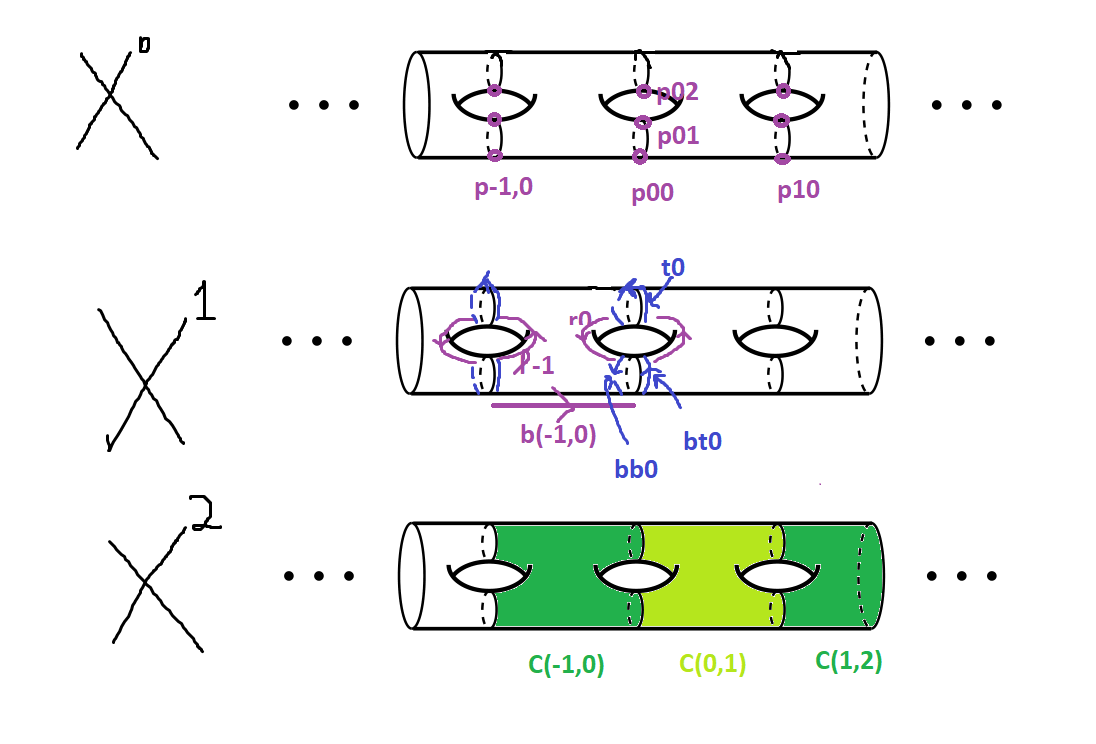
\includegraphics[width=\linewidth]{mt1}
\end{figure}

Now, we apply the recipe to compute the fundamental group of this image.

The first thing we need to do is fix a spanning tree of the graph $X^1$. Once we do, the generators of the fundamental group are (in one-to-one correspondence with) the edges of the graph which are not in this spanning tree. We choose the spanning tree given by all edges of the forms: $b_{i(i+1)}$, $bb_i$, and $r_i$. Therefore, the generators of the fundamental group are $t_{i(i+1)}$, $bt_i$, $\ell_i$, and $t_i$.

Now, the relations of the fundamental group are given by the two-cells. In this case, each cell $C(i,i+1)$ will furnish a relation between the generators $bt_i$, $bt_{i+1}$, $\ell_i$, $t_i$, and $t_{i+1}$. In order to understand what these relations are, we will now draw a cell $C(i,i+1)$ with its attaching map.
\begin{figure}[H]
\centering
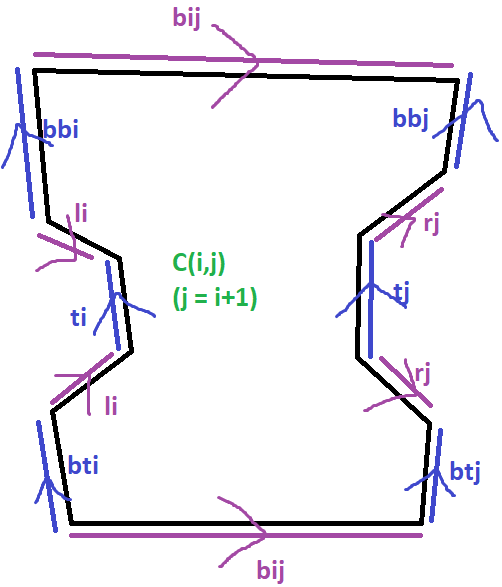
\includegraphics[width=5cm]{mt2}
\end{figure}

Now, each relation consists of going `around the attaching map' once, and identifying the resulting path with zero. We do this with this cell. Each edge in the spanning tree is ignored. The other edges correspond to their namesake generator. We obtain the relation: (with $j = i+1$)
\begin{equation} \label{eq:rels}
bt_j \, t_j \, \ell_i \, t_i^{-1} \, \ell_i^{-1} \, bt_i^{-1} = e.
\end{equation}

Now, this relation lets us write $bt_{i+1}$ in terms of the $t_j$, $\ell_j$, and in terms of $bt_i$, and the reverse could be done. Therefore, \emph{we may write all $bt_i$ in terms of the $t_j$, $\ell_j$, and $bt_0$}.\footnote{I could write the explicit expression, but I don't think it's necessary. To convince the reader that I know what I'm doing, however, I will sketch the expression for $bt_n$ with $n \geq 0$: $bt_n = bt_0 \ell_0 t_0 \ell_0^{-1} t_1 \dots \ell_{n-1} t_{n-1} \ell_{n-1}^{-1} t_n$.} This suggests that we consider instead these generators.

So, we consider the obvious map
\begin{equation}\label{eq:iso}
\braket{bt_0, t_i, \ell_i} \to \braket{bt_i, t_i, \ell_i \mid \eqref{eq:rels}}.
\end{equation}

We claim that this map is an isomorphism, because the inverse is well-defined. Indeed, to define the inverse, we need only take each $t_i$ and $\ell_i$ to itself, and each $bt_i$ to the expression that writes it in terms of the other generators. All that we need to show is that this correspondence respects the relations \eqref{eq:rels}; once we do we will have an inverse.

Showing that this correspondence respects \eqref{eq:rels} is trivially done by induction on $i$ (twice; once for positive $i$ and once for negative), and boils down to the fact that the expression we are sending each $bt_i$ to is precisely what makes \eqref{eq:rels} hold.

Since the map \eqref{eq:iso} is an isomorphism between a free group on countably many generators and a group which is isomorphic to the free group of the space under consideration, the exercise is solved.

\smallskip

Another way to see this solution: inductively we rewrite the equations \eqref{eq:rels} to all be of the form $bt_n = (\cdots)$, where the expression on the right-hand side depends only on the generators we've been discussing, and then we may simply remove all the generators $bt_n$, $n \neq 0$, together with the relations that tell us how to write them in terms of the others; this preserves the group up to isomorphism because adding generators and relations telling us how to write these generators in terms of the previous ones does not add any elements or identifications to the group.
\end{sol}

\begin{ex}[1.3:9]
Show that if a path-connected, locally path-connected space $X$ has finite fundamental group, then every map $f \colon X \to S^1$ is nulhomotopic.
\end{ex}

\begin{sol}
Pick a basepoint $x \in X$, and $* = f(x)$. Then, $f$ induces a homomorphism $f_* \colon \pi(X,x) \to \pi(S^1,*) \cong \Z$. Then, $f_*$ must be the zero map, because the image of $f_*$ must be a finite subgroup of $\Z$, the only one of which is the zero subgroup.

As a consequence, the map $f$ lifts to a map $\tilde f \colon X \to \R$, as $f_*(\pi(X,x)) = 0 \subseteq p_*(\pi(\R))$. Since $\R$ is contractible, $\tilde f$ is nulhomotopic, and composing this homotopy with $p \colon \R \to S^1$ yields a homotopy between $f$ and a constant map.
\end{sol}

\begin{ex}[1.B:2]
Let $X$ be a connected CW complex and $G$ a group such that every homomorphism $\pi(X) \to G$ is trivial. Show that every map $X \to K(G,1)$ is nulhomotopic.
\end{ex}

\begin{sol}
I mean... You just repeat the argument in the previous exercise right? It follows through, word for word, you just have to replace $S^1$ with $K(G,1)$ and $\R$ with the universal cover of this space. Everything follows because connected CW complexes are Very Nice (locally path connected, and path connected in our case, so the map lifting property applies) and the universal cover of $K(G,1)$ is contractible by definition.
\end{sol}

\begin{ex}[2.1:5]
Compute the simplicial homology groups of the Klein bottle using the $\Delta$-complex furnished by Hatcher.
\end{ex}

\begin{sol}
By looking at the figure on page 102 of hatcher, we see that the chain complex of this $\Delta$-complex is given as follows:
\begin{gather}
C_0 = \braket{v},\\
C_1 = \braket{a,b,c},\\
C_2 = \braket{U,L},
\end{gather}
which already tells us that the zeroth homology is $H_0 = C_0 = \braket{v} \cong \Z$.

The boundary maps on $C_1$ and $C_2$ are given by
\begin{gather}
\partial(a) = \partial(b) = \partial(c) = 0,\\
\partial(U) = b - c + a, \quad \partial(L) = a - b + c.
\end{gather}

Therefore, $Z_1 = \braket{a,b,c}$ and $B_1 = \braket{b-c+a, a-b+c} = \braket{2a,a-b+c}$. Thus, $H_1$ is presented as
\begin{equation}
H_1 \cong \braket{a,b,c \mid 2a = e, a = b-c}.
\end{equation}

Now, in this presentation it is obvious that we can remove the generator $a$, and obtain the presentation
\begin{equation}
H_1 \cong \braket{b,c \mid 2b = 2c}.
\end{equation}

If instead of the generators $b$ and $c$ we use the generators $b$ and $z = c-b$, we obtain instead
\begin{equation}
H_1 \cong \braket{b,z \mid 2z = 0} \cong \Z \oplus \Z/2,
\end{equation}
which completes the computation of the first simplicial homology.

Finally, the second simplicial homology is just the kernel of $\partial \colon C_2 \to C_1$. To this effect, we find the pairs of integers $x,y$ for which
\begin{equation}
\begin{aligned}
& \partial(xU + yL) = 0\\
\iff & (x+y) a + (x - y)b + (y-x) c = 0\\
\iff & x+y = 0 \text{ and } x-y = 0,
\end{aligned}
\end{equation}
and this equation can easily be solved to yield $x = y = 0$. Thus, $Z_2 = 0$ and hence $H_2 = 0$.
\end{sol}

\begin{ex}[2.2:12]
Show that the quotient map $q \colon T \to S^2$ which collapses $S^1 \vee S^1$ to a point is not nulhomotopic by showing that it is an isomorphism on $H_2$. On the other hand, show that any map $S^2  \to T$ is nulhomotopic.
\end{ex}

\begin{sol}
We use the long exact sequence. Since $(T,S^1 \vee S^1)$ is a CW pair, it is a good pair, hence we have that this sequence is exact:
\begin{equation}
H_2(S^1 \vee S^1) \to H_2(T) \xrightarrow{q_*} H_2(S^2) \xrightarrow{\partial} H_1(S^1 \vee S^1) \xrightarrow{i_*} H_1(T)
\end{equation}

Now, using simplicial or cellular homology we see trivially that $H_2(S^1 \vee S^1$ is null, whence $q_*$ is injective.

We note that injectivity of $q_*$ is enough to show that the quotient map is not nulhomotopic, but the exercise asks to show that it is a homomorphism, so we proceed.

We see that surjectivity of $q_*$ is equivalent to $\partial$ being null, which is equivalent to $i_*$ being surjective. Now, this can be verified by using simplicial homology, using the standard $\Delta$-complexes on $S^1 \vee S^1$ and $T$. Indeed, since the inclusion $i \colon S^1 \vee S^1 \to T$ is the inclusion of the one-skeleton of $T$ in its two skeleton, we obtain that $i_*$ is a quotient map, which is evidently surjective. (It's actually an isomorphism but we don't need that right now.)

Anyway, this finishes the proof that $q_*$ is an isomorphism of abelian groups.

\medskip

Now, let $f \colon S^2 \to T$. Since $S^2$ is simply connected and Very Nice, $f$ lifts to a map to the universal covering of $T$, which is $\R^2$. This lift is nulhomotopic, and composing it with $p \colon \R^2 \to T$ we conclude that $f$ itself is nulhomotopic.
\end{sol}

\begin{ex}[2.2:29]
[Note: This solution was written before I saw that the exercise had changed, but Danny let me submit it regardless.]

Compute the homology groups of $X$ using the Mayer-Vietoris sequence for the given decomposition of $X$ into two copies of $R$. Compute also the relative groups $H_i(R,M)$ with $M = M_g$.
\end{ex}

\begin{sol}
We begin by noting that $(X,M)$ is a good pair, because $(R, M)$ is a good pair. Let $U$ be a neighborhood of $M$ in $X$ which deformation retracts to $M$. Now, let $A = R \cup U$ and $B = R \cup U$, where each of them refers to a distinct copy of $R \subseteq X$. I know the notation is silly, but I'm sure the reader will understand what I mean.

Now, $X = A \cup B$ and both $A$ and $B$ are open, so the Mayer-Vietoris sequence applies
\begin{equation}
\cdots \to H_n(A \cap B) \to H_n(A) \oplus H_n(B) \to H_n(X) \to H_{n-1}(A \cap B) \to \cdots
\end{equation}

Now, note that $A$ and $B$ are both homotopically equivalent to $R$, which retracts by deformation to a wedge of $g$ circles,, and $A \cap B$ is homotopically equivalent to $M$. This means that we know pretty well the homologies of $A$, $B$, and $A \cap B$:
\begin{equation}
\begin{aligned}
H_n(A) \cong H_n(B) &\cong \begin{cases}
0 & \text{if $n > 1$,}\\
\Z^g & \text{if $n = 1$,}\\
\Z & \text{if $n = 0$,}
\end{cases}\\
H_n(A \cap B) &\cong \begin{cases}
0 & \text{if $n > 2$,}\\
\Z & \text{if $n = 2$,}\\
\Z^{2g} & \text{if $n = 1$,}\\
\Z & \text{if $n = 0$,}
\end{cases}
\end{aligned}
\end{equation}
where the computation of $H_n(A \cap B) \cong H_n(M)$ is done in example 2.36 of Hatcher.

With this data, we see that the Mayer-Vietoris sequence looks like
\begin{equation}
\begin{aligned}
\cdots &\to 0 \to 0 \oplus 0 \to H_3(X) \to \\
&\to \Z \to 0 \oplus 0 \to H_2(X) \to\\
&\to \Z^{2g} \to \Z^{g} \oplus \Z^{g} \to H_1(X) \to\\
&\to \Z \to \Z \oplus \Z \to H_0(X) \to 0.
\end{aligned}
\end{equation}

We see immediately that $H_3(X) \cong \Z$. Moreover, $H_2(X)$ is identified with a subgroup of $\Z^{2g}$, namely the kernel of the map $\Z^{2g} \to \Z^g \oplus \Z^g$, so we had better find out what this map is.

This map has two components, each of which is induced by the inclusion $M \hookrightarrow R$. This can be seen as an inclusion of CW complexes, but it is not an inclusion of the two-skeleton into the three-skeleton. To make it work, we need to first `slice $R$ up into a bunch of balls'. To see what this means, see the following figure.
\begin{figure}[H]
\centering
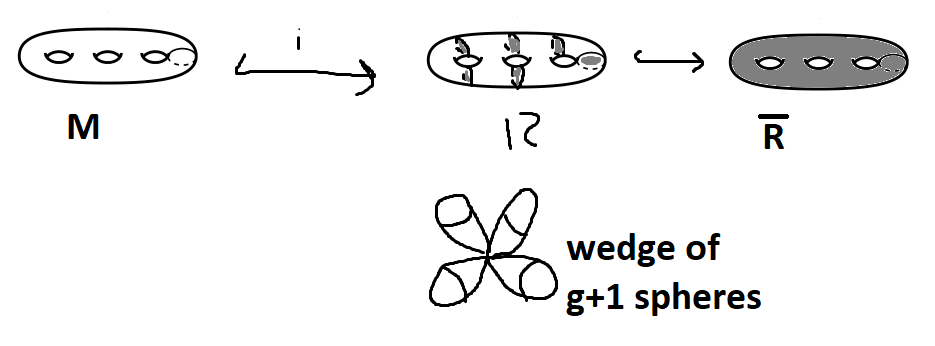
\includegraphics[width=\linewidth]{mt3}
\end{figure}

Now, note that the wedge of $g+1$ spheres has null first homology, hence $i_* = 0$, and by functoriality the map $\Z^{2g} \to \Z^g$ is null. As a consequence, $H_2(X) \cong \Z^{2g}$, and moreover we have the exact sequence
\begin{equation}
\xrightarrow{0} \Z^g \oplus \Z^g \to H_1(X) \to \Z \to \Z \oplus \Z \to (H_0(X) \cong \Z) \to 0,
\end{equation}
where $H_0(X)$ is isomorphic to $\Z$ because $X$ is path connected and nonempty.

Now, if we can show that the map $\Z \to \Z \oplus \Z$ is null, we have the exercise done. We could do this directly, but instead we will use the following trick: use Mayer-Vietoris for reduced homology instead! If we do this, the zeroth homology of $A \cap B$ becomes null, and we instead have the exact sequence
\begin{equation}
\xrightarrow{0} \Z^g \oplus \Z^g \to H_1(X) \to 0,
\end{equation}
which proves that $H_1 \cong \Z^g \oplus \Z^g \cong \Z^{2g}$. This completes the computation of the homology of $X$:
\begin{equation}
H_n(X) \cong \begin{cases}
0 & \text{if $n > 3$,}\\
\Z & \text{if $n = 3$,}\\
\Z^{2g} & \text{if $n = 2$,}\\
\Z^{2g} & \text{if $n = 1$,}\\
\Z & \text{if $n = 0$.}
\end{cases}
\end{equation}

\medskip

Now, to compute the relative groups, we use the long exact sequence for the pair $(R,M)$. It looks very similar, because where before we had $H_n(A \cap B)$ we now have the isomorphic $H_n(M)$, and where we had $H_n(A) \oplus H_n(B) \cong H_n(R) \oplus H_n(R)$ we now have just $H_n(R)$.
\begin{equation}
\begin{aligned}
\cdots &\to 0 \to 0 \to H_3(R,M) \to \\
&\to \Z \to 0 \to H_2(R,M) \to\\
&\to \Z^{2g} \to \Z^{g} \to H_1(R,M) \to\\
&\to \Z \to \Z \to H_0(R,M) \to 0.
\end{aligned}
\end{equation}

Now, the same arguments that before showed that certain maps were null still hold, and therefore we have, by exactly the same reasons,
\begin{equation}
H_n(R,M) \cong \begin{cases}
0 & \text{if $n > 3$,}\\
\Z & \text{if $n = 3$,}\\
\Z^{2g} & \text{if $n = 2$,}\\
\Z^{g} & \text{if $n = 1$,}\\
\Z & \text{if $n = 0$.}
\end{cases}
\end{equation}
\end{sol}

\end{document}